\documentclass[12pt]{article}

% Template SBC: baixe sbc-template.sty e sbc.bst (https://www.sbc.org.br/documentos-da-sbc/)
% e coloque nesta pasta. Se o professor exigir IEEE, avise para trocar o preambulo.
\usepackage{sbc-template}
\usepackage{graphicx,url}
\usepackage[utf8]{inputenc}
\usepackage[T1]{fontenc}
\usepackage[brazil]{babel}
\usepackage{booktabs}

\sloppy

\title{An\'alise Experimental de Algoritmos de Ordena\c{c}\~ao\\sobre Avalia\c{c}\~oes do MovieLens 25M}

\author{Henrique Balassa\inst{1}, Laura Veiga\inst{1}, Saulo Resende\inst{1}} % TODO: sobrenomes completos

\address{Instituto Federal Catarinense -- Campus S\~ao Bento do Sul\\
  Curso de Engenharia de Computa\c{c}\~ao -- Estrutura de Dados\\
  S\~ao Bento do Sul -- SC -- Brasil
  \email{\{emails institucionais\}@...} % TODO
}

\begin{document}
\maketitle

\begin{abstract}
This paper presents an experimental comparison of four sorting algorithms (Insertion Sort, Selection Sort, Quick Sort with three pivot strategies, and Merge Sort) applied to up to one million ratings from the MovieLens 25M dataset. We measured running time, key comparisons and element moves for two sort keys and three input orderings. Results confirm the theoretical classes, but also show that the pivot choice can turn Quick Sort into a quadratic algorithm on already-ordered data, and that Merge Sort, despite performing fewer comparisons, was slower than Quick Sort on random data.
\end{abstract}

\begin{resumo}
Este artigo compara experimentalmente quatro algoritmos de ordena\c{c}\~ao (Insertion Sort, Selection Sort, Quick Sort com tr\^es estrat\'egias de piv\^o e Merge Sort) aplicados a at\'e um milh\~ao de avalia\c{c}\~oes do conjunto MovieLens 25M. Foram medidos tempo de execu\c{c}\~ao, compara\c{c}\~oes de chaves e movimenta\c{c}\~oes de elementos para duas chaves de ordena\c{c}\~ao e tr\^es disposi\c{c}\~oes de entrada. Os resultados confirmam as classes de complexidade te\'oricas, mas mostram que a escolha do piv\^o pode tornar o Quick Sort quadr\'atico em dados j\'a ordenados e que o Merge Sort, apesar de fazer menos compara\c{c}\~oes, foi mais lento que o Quick Sort em dados aleat\'orios.
\end{resumo}

\section{Introdu\c{c}\~ao}

A ordena\c{c}\~ao \'e uma das opera\c{c}\~oes mais frequentes em sistemas de software e serve de base para busca, agrupamento e remo\c{c}\~ao de duplicatas \cite{cormen2012}. Algoritmos com a mesma finalidade podem ter custos muito diferentes conforme o tamanho e a disposi\c{c}\~ao dos dados, o que torna a an\'alise assint\'otica necess\'aria, mas n\~ao suficiente: constantes, uso de mem\'oria e comportamento do hardware tamb\'em pesam.

Este trabalho compara experimentalmente Insertion Sort, Selection Sort, Quick Sort e Merge Sort sobre dados reais. O objetivo \'e verificar at\'e que ponto o comportamento medido segue a teoria e identificar em que situa\c{c}\~oes cada algoritmo \'e adequado. Todas as implementa\c{c}\~oes foram escritas pelo grupo em Java, sem uso de m\'etodos de ordena\c{c}\~ao da biblioteca padr\~ao nas medi\c{c}\~oes.

\section{Fundamenta\c{c}\~ao Te\'orica}

A Tabela~\ref{tab:teoria} resume as complexidades de tempo (n\'umero de compara\c{c}\~oes) e propriedades dos algoritmos \cite{cormen2012,ziviani2007,knuth1998}.

\begin{table}[ht]
\centering
\caption{Complexidade e propriedades dos algoritmos estudados.}
\label{tab:teoria}
\begin{tabular}{lcccccc}
\toprule
Algoritmo & Melhor & M\'edio & Pior & Est\'avel & Mem\'oria extra \\
\midrule
Insertion Sort & $O(n)$ & $O(n^2)$ & $O(n^2)$ & sim & $O(1)$ \\
Selection Sort & $O(n^2)$ & $O(n^2)$ & $O(n^2)$ & n\~ao & $O(1)$ \\
Quick Sort & $O(n\log n)$ & $O(n\log n)$ & $O(n^2)$ & n\~ao & $O(\log n)$ \\
Merge Sort & $O(n\log n)$ & $O(n\log n)$ & $O(n\log n)$ & sim & $O(n)$ \\
\bottomrule
\end{tabular}
\end{table}

O Insertion Sort insere cada elemento na parte j\'a ordenada e, por isso, faz apenas $n-1$ compara\c{c}\~oes em uma entrada ordenada. O Selection Sort sempre faz $n(n-1)/2$ compara\c{c}\~oes, independentemente da entrada, mas no m\'aximo $n-1$ trocas. O Merge Sort divide o vetor ao meio, ordena cada metade e intercala, garantindo $O(n\log n)$ em qualquer caso ao custo de um vetor auxiliar.

O Quick Sort \cite{hoare1962} particiona o vetor em torno de um piv\^o e ordena recursivamente as partes. Seu desempenho depende de o piv\^o dividir bem o vetor: se o piv\^o \'e sempre o menor ou o maior elemento, as parti\c{c}\~oes ficam desbalanceadas e o custo vira $O(n^2)$. Foram avaliadas tr\^es estrat\'egias: primeiro elemento, mediana de tr\^es (primeiro, meio e \'ultimo) e piv\^o aleat\'orio.

\section{Metodologia}

\paragraph{Dados.} Foi usado o MovieLens 25M \cite{harper2015}, que cont\'em 25 milh\~oes de avalia\c{c}\~oes. Sorteamos 1.000.000 de registros (semente 2026) e os embaralhamos; as amostras de 10.000 e 100.000 s\~ao prefixos dessa amostra. Cada registro cont\'em usu\'ario, filme, nota e \emph{timestamp}.

\paragraph{Chaves e entradas.} Ordenamos por duas chaves: \emph{timestamp} (973.187 valores distintos na amostra de 1 milh\~ao) e nota (apenas 10 valores distintos, de 0,5 a 5,0), para observar o efeito de chaves quase \'unicas versus muito repetidas. Cada chave foi testada em tr\^es disposi\c{c}\~oes: j\'a ordenada, em ordem reversa e aleat\'oria.

\paragraph{Implementa\c{c}\~ao e m\'etricas.} As implementa\c{c}\~oes s\~ao do grupo; o Quick Sort usa parti\c{c}\~ao de Hoare e recorre apenas sobre a menor parte, limitando a pilha a $O(\log n)$. Todas as compara\c{c}\~oes passam por um \'unico m\'etodo, que as conta; contamos como movimenta\c{c}\~ao cada escrita no vetor (uma troca vale duas). A corre\c{c}\~ao de cada sa\'ida foi verificada contra as chaves de refer\^encia ordenadas, e o conjunto de testes automatizados (108.000 casos, incluindo estabilidade) passou.

\paragraph{Ambiente e procedimento.} Os experimentos rodaram em AMD64 Family 25 Model 80 (16 processadores l\'ogicos, 15.774 MB de RAM), Windows 11, Java 26.0.2 (HotSpot), em 22/11/2026. Antes das medi\c{c}\~oes, uma execu\c{c}\~ao de aquecimento com 20.000 registros reduz o efeito da compila\c{c}\~ao JIT, e \texttt{System.gc()} \'e chamado antes de cada execu\c{c}\~ao. Cada caso foi repetido 5 vezes e reportamos m\'edia $\pm$ desvio-padr\~ao amostral; execu\c{c}\~oes acima de 20 s n\~ao foram repetidas. Para tratar algoritmos quadr\'aticos, impusemos um limite de 120 s por execu\c{c}\~ao: ao estourar, a execu\c{c}\~ao \'e interrompida e registrada como ``$>$ 120 s''.

\section{Resultados}

As Tabelas~\ref{tab:tempo-timestamp-100000} e~\ref{tab:tempo-timestamp-1000000} trazem os tempos para a chave \emph{timestamp}; a Tabela~\ref{tab:comp-timestamp-100000} traz as compara\c{c}\~oes com $n=100.000$. As demais combina\c{c}\~oes (chave nota e $n=10.000$) est\~ao no reposit\'orio do trabalho. A Figura~\ref{fig:tempo} mostra o tempo em fun\c{c}\~ao de $n$, e a Figura~\ref{fig:pivo} compara os tr\^es piv\^os.

\begin{table}[ht]
\centering
\caption{Tempo de ordena\c{c}\~ao (ms), chave timestamp, n = 100.000. M\'edia $\pm$ desvio-padr\~ao de 5 repeti\c{c}\~oes. * = execu\c{c}\~ao \'unica (acima de 20 s n\~ao se repete). $>$ 120 s = execu\c{c}\~ao interrompida no limite de tempo. }
\label{tab:tempo-timestamp-100000}
\begin{tabular}{lrrr}
\hline
Algoritmo & Ordenado & Reverso & Aleat\'orio \\
\hline
Insertion Sort & 2,35 $\pm$ 0,30 & 30.615* & 14.988 $\pm$ 96,4 \\
Selection Sort & 23.448* & 23.007* & 19.109 $\pm$ 958,4 \\
Quick Sort (piv\^o: primeiro) & 21.787* & 29.835* & 26,6 $\pm$ 0,71 \\
Quick Sort (piv\^o: mediana de tr\^es) & 12,1 $\pm$ 0,05 & 13,2 $\pm$ 0,32 & 26,1 $\pm$ 0,49 \\
Quick Sort (piv\^o: aleat\'orio) & 18,2 $\pm$ 0,29 & 19,5 $\pm$ 0,96 & 27,9 $\pm$ 0,54 \\
Merge Sort & 11,9 $\pm$ 0,36 & 15,6 $\pm$ 0,21 & 29,5 $\pm$ 0,69 \\
\hline
\end{tabular}
\end{table}

\begin{table}[ht]
\centering
\caption{Tempo de ordena\c{c}\~ao (ms), chave timestamp, n = 1.000.000. M\'edia $\pm$ desvio-padr\~ao de 5 repeti\c{c}\~oes. * = execu\c{c}\~ao \'unica (acima de 20 s n\~ao se repete). $>$ 120 s = execu\c{c}\~ao interrompida no limite de tempo. }
\label{tab:tempo-timestamp-1000000}
\begin{tabular}{lrrr}
\hline
Algoritmo & Ordenado & Reverso & Aleat\'orio \\
\hline
Insertion Sort & 33,9 $\pm$ 0,30 & $>$ 120 s & $>$ 120 s \\
Selection Sort & $>$ 120 s & $>$ 120 s & $>$ 120 s \\
Quick Sort (piv\^o: primeiro) & $>$ 120 s & $>$ 120 s & 311,6 $\pm$ 2,46 \\
Quick Sort (piv\^o: mediana de tr\^es) & 130,8 $\pm$ 36,1 & 142,9 $\pm$ 2,36 & 319,8 $\pm$ 2,10 \\
Quick Sort (piv\^o: aleat\'orio) & 164,9 $\pm$ 1,00 & 190,7 $\pm$ 1,52 & 324,8 $\pm$ 0,75 \\
Merge Sort & 216,2 $\pm$ 7,05 & 265,3 $\pm$ 1,34 & 444,8 $\pm$ 6,66 \\
\hline
\end{tabular}
\end{table}

\begin{table}[ht]
\centering
\caption{Compara\c{c}\~oes entre chaves, chave timestamp, n = 100.000. -- = execu\c{c}\~ao interrompida (contagem incompleta, n\~ao compar\'avel).}
\label{tab:comp-timestamp-100000}
\begin{tabular}{lrrr}
\hline
Algoritmo & Ordenado & Reverso & Aleat\'orio \\
\hline
Insertion Sort & 99.999 & 4.999.949.982 & 2.509.842.849 \\
Selection Sort & 4.999.950.000 & 4.999.950.000 & 4.999.950.000 \\
Quick Sort (piv\^o: primeiro) & 4.999.887.741 & 4.979.847.622 & 2.657.217 \\
Quick Sort (piv\^o: mediana de tr\^es) & 2.047.510 & 2.047.529 & 2.613.307 \\
Quick Sort (piv\^o: aleat\'orio) & 2.540.017 & 2.534.509 & 2.434.960 \\
Merge Sort & 853.904 & 815.271 & 1.536.417 \\
\hline
\end{tabular}
\end{table}


\begin{figure}[ht]
\centering
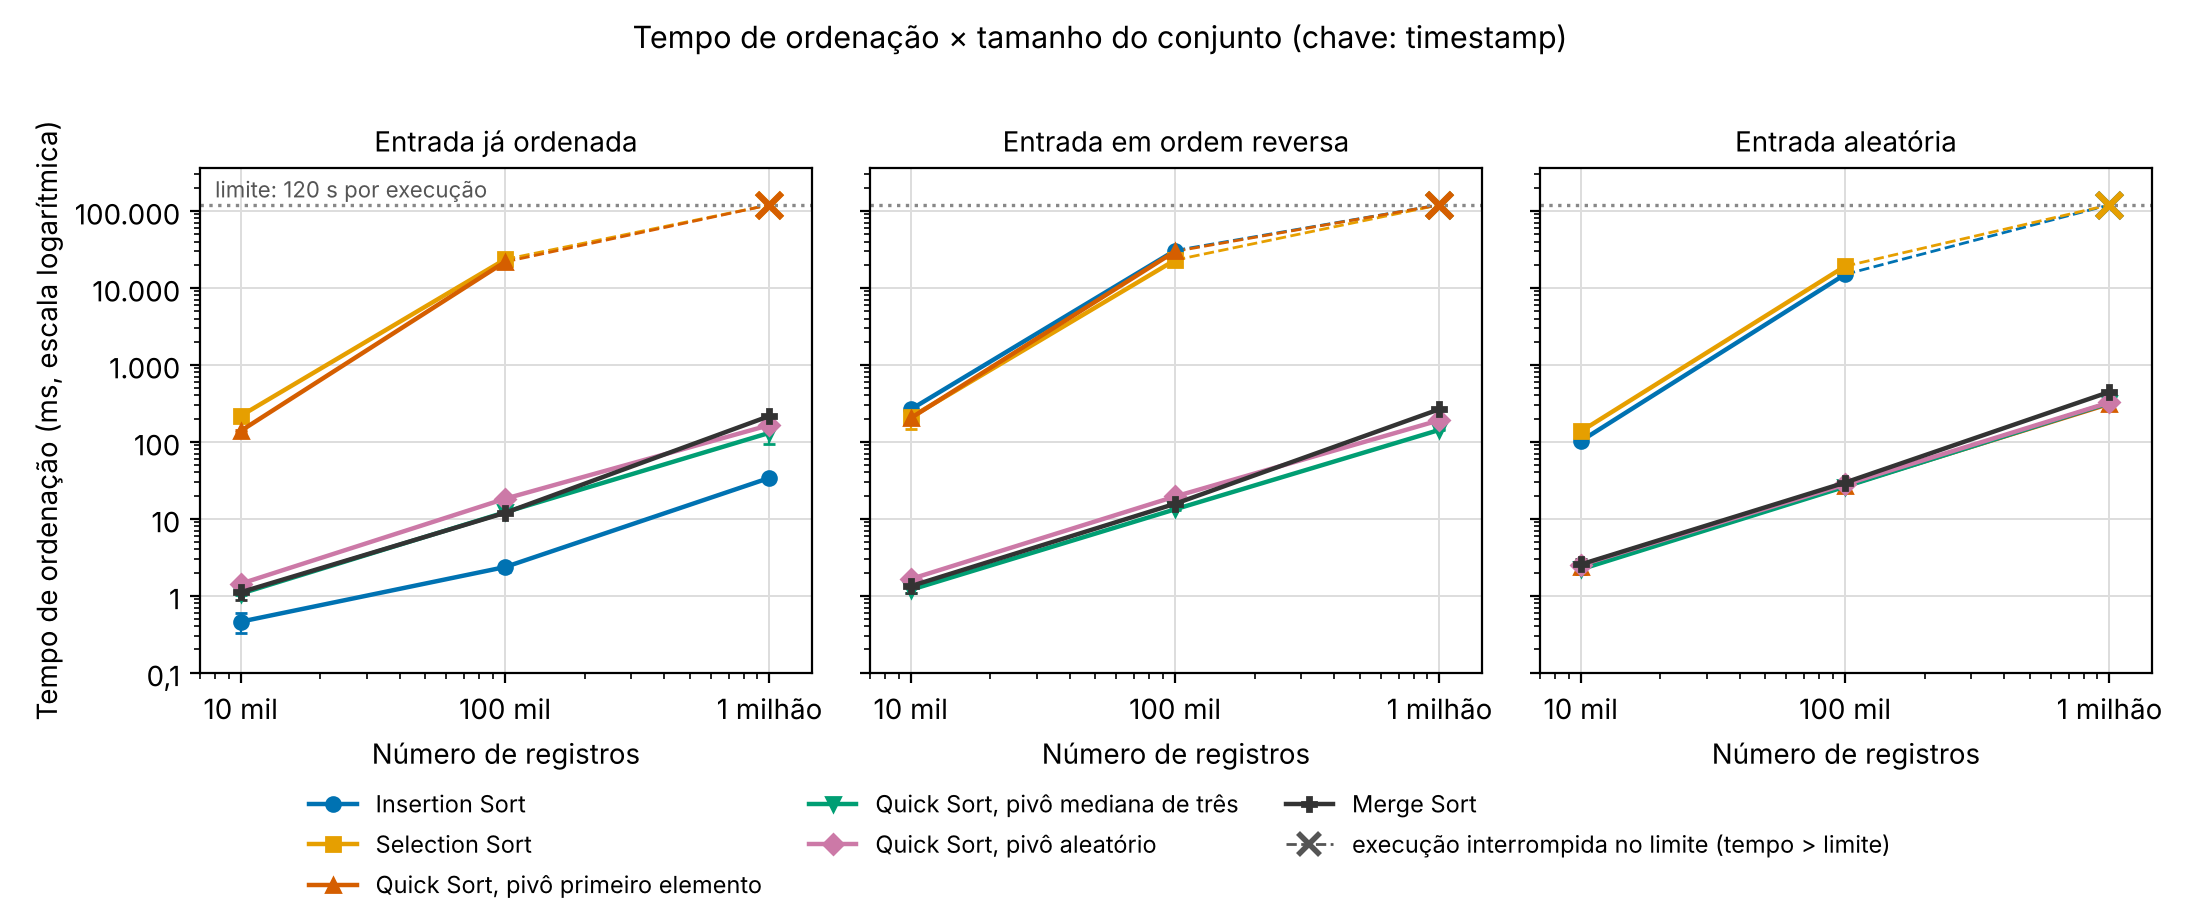
\includegraphics[width=\textwidth]{tempo_timestamp.png}
\caption{Tempo de ordena\c{c}\~ao em fun\c{c}\~ao de $n$ (chave \emph{timestamp}, escala logar\'itmica).}
\label{fig:tempo}
\end{figure}

\begin{figure}[ht]
\centering
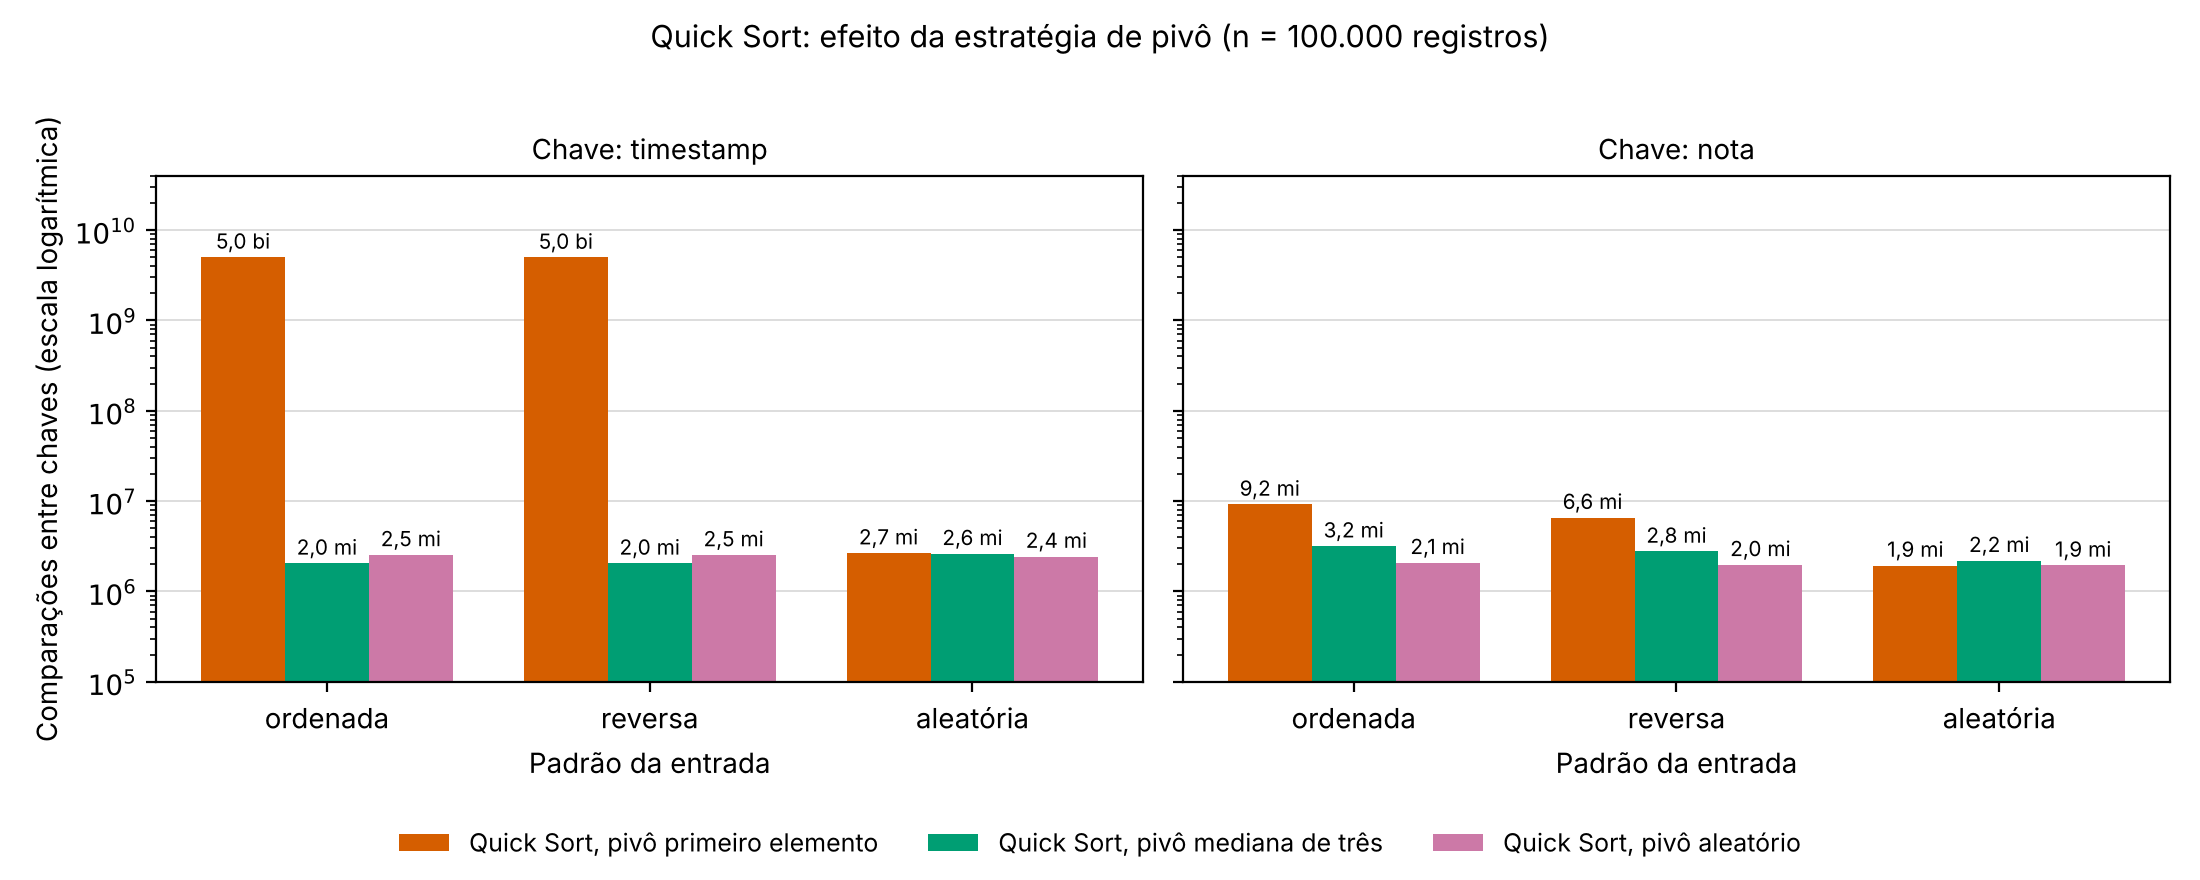
\includegraphics[width=.9\textwidth]{quicksort_pivo.png}
\caption{Quick Sort com diferentes piv\^os, $n=100.000$.}
\label{fig:pivo}
\end{figure}

\section{Discuss\~ao}

\paragraph{Teoria versus pr\'atica.} As classes previstas aparecem nos dados. O Selection Sort fez exatamente $n(n-1)/2 = 4.999.950.000$ compara\c{c}\~oes com $n=100.000$ em qualquer disposi\c{c}\~ao, e levou cerca de 19 a 23 s. O Insertion Sort fez 99.999 compara\c{c}\~oes e levou 2,35 ms na entrada ordenada, mas 2,5 bilh\~oes de compara\c{c}\~oes e cerca de 15 s na aleat\'oria. Nos algoritmos $O(n\log n)$, o Merge Sort passou de $n=100.000$ para $n=1.000.000$ com custo multiplicado por cerca de 15 (esperado: aproximadamente 12).

\paragraph{O piv\^o importa.} Com o primeiro elemento como piv\^o, o Quick Sort ordenou 100.000 registros aleat\'orios em 26,6 ms, mas levou 21,8 s na entrada j\'a ordenada, com 4.999.887.741 compara\c{c}\~oes: o pior caso quadr\'atico. A mediana de tr\^es resolveu isso (12,1 ms) e o piv\^o aleat\'orio tamb\'em (18,2 ms). Com $n=1.000.000$, o piv\^o ``primeiro'' foi interrompido em 120 s nas entradas ordenada e reversa. Na chave nota, com poucos valores distintos, o mesmo piv\^o tamb\'em se degradou (874 ms contra 305 ms da mediana de tr\^es em $n=1.000.000$, entrada ordenada).

\paragraph{Quick Sort versus Merge Sort.} O Merge Sort fez menos compara\c{c}\~oes (18,7 milh\~oes contra cerca de 30 milh\~oes em $n=1.000.000$ aleat\'orio), mas foi mais lento (444,8 ms contra cerca de 320 ms). Uma poss\'ivel explica\c{c}\~ao, que n\~ao testamos diretamente, \'e o custo de mover dados e usar o vetor auxiliar: o Merge Sort fez cerca de 29,4 milh\~oes de movimenta\c{c}\~oes contra 9 a 11 milh\~oes do Quick Sort. Em contrapartida, o Merge Sort tem tempo mais previs\'ivel e \'e est\'avel.

\paragraph{Limite dos algoritmos quadr\'aticos.} Com $n=1.000.000$, o Selection Sort foi interrompido em todas as combina\c{c}\~oes. Em 120 s ele alcan\c{c}ou entre 6,6 e 29,3 bilh\~oes de compara\c{c}\~oes, de cerca de $5\times10^{11}$ necess\'arias; extrapolando, a execu\c{c}\~ao completa levaria algo entre 34 minutos e 2,5 horas (estimativa, n\~ao medi\c{c}\~ao). O Insertion Sort s\'o terminou na entrada ordenada (33,9 ms). Assim, para ordena\c{c}\~ao geral nessa escala, algoritmos quadr\'aticos s\~ao invi\'aveis; o Insertion Sort s\'o se justifica para vetores pequenos ou quase ordenados.

\paragraph{Limita\c{c}\~oes.} Os tempos com $n=10.000$ s\~ao ruidosos por causa do JIT; a mem\'oria n\~ao foi medida; as medi\c{c}\~oes vieram de uma \'unica m\'aquina; e uma execu\c{c}\~ao (Insertion Sort, nota, aleat\'oria, $n=1.000.000$) registrou tempo an\^omalo e foi tratada como ``$>$ 120 s''.

\section{Conclus\~ao}

Os experimentos confirmaram a an\'alise te\'orica e mostraram que detalhes de implementa\c{c}\~ao, como o piv\^o do Quick Sort, mudam a ordem de grandeza do custo. Para dados grandes e de disposi\c{c}\~ao desconhecida, Quick Sort com mediana de tr\^es ou piv\^o aleat\'orio foi a op\c{c}\~ao mais r\'apida; o Merge Sort \'e prefer\'ivel quando se precisa de estabilidade ou de tempo previs\'ivel; o Insertion Sort serve para vetores pequenos ou quase ordenados; e o Selection Sort n\~ao se mostrou competitivo. Como trabalho futuro, sugerem-se medir mem\'oria, comparar com a ordena\c{c}\~ao da biblioteca padr\~ao e repetir os testes em outras m\'aquinas.

\section*{Declara\c{c}\~ao de uso de ferramentas de IA}

% TODO: confirmar com o grupo e ajustar ao que de fato ocorreu.
Foi utilizado o assistente Claude (Anthropic) como apoio em: programa\c{c}\~ao e testes das implementa\c{c}\~oes, pesquisa de fontes e revis\~ao do texto. O grupo revisou e executou todo o c\'odigo e \'e respons\'avel pelos resultados e pelas conclus\~oes apresentadas.

\bibliographystyle{sbc}
\bibliography{refs}

\end{document}
